\documentclass[11pt]{beamer}
\usepackage{amsmath}
\usepackage{amssymb}
\usepackage{geometry}
\usepackage{graphicx}
\usepackage{url}
\usepackage{xcolor}
\usepackage{enumerate}

% some latex magic for correcting apostrophe issue in verbatim mode
\makeatletter
\let \@sverbatim \@verbatim
\def \@verbatim {\@sverbatim \verbatimplus}
{\catcode`'=13 \gdef \verbatimplus{\catcode`'=13 \chardef '=13 }} 
\makeatother

\begin{document}

%---------------------------------------------
\begin{frame}
\large
Lecture 7:\\
Confidence Intervals for a Proportion\\
STAT 310, Spring 2021
\normalsize
\end{frame}

%---------------------------------------------
\begin{frame}{Introduction}
\begin{itemize}
\item A \textbf{point estimate} is our best guess of the value of a population parameter based on a random sample of data.
\vspace{5pt}
\begin{itemize}
\item $\hat{p}$ is a point estimate $p$
\vspace{5pt}
\item $\bar{x}$ is a point estimate $\mu$
\end{itemize}
\vspace{10pt}
\item An \textbf{confidence interval} gives a range of plausible values for the population parameter.
\end{itemize}
\end{frame}

%---------------------------------------------
\begin{frame}{Confidence Interval for $p$}
\vspace{-1.5cm}
A 95\% confidence interval for the population proportion $p$ is given by the formula\\
\vspace{5pt}
$$\hat{p} \pm 1.96 \sqrt{\frac{\hat{p}(1-\hat{p})}{n}}$$
\end{frame}

%---------------------------------------------
\begin{frame}{Confidence Interval for $p$}
The confidence interval formula is valid if the following conditions are satisfied:
\begin{itemize}
\vspace{5pt}
\item The data were collected using simple random sampling.  This is called the \textbf{independence} condition.
\vspace{5pt}
\item $n \hat{p} \geq 10$ and $n (1-\hat{p}) \geq 10$.  This is called the \textbf{success-failure} condition.
\end{itemize}
\vspace{5pt}
These conditions ensure that the Central Limit Theorem holds, and so the sampling distribution for $\hat{p}$ is approximately normal.
\end{frame}

%---------------------------------------------
\begin{frame}{Example}
\small
A recent Gallup poll estimated that 56\% of Americans approved of the way Joe Biden is handling his job as president.  The results were based on a random sample of 1,202 American adults.\footnote{\tiny \url{https://news.gallup.com/poll/329948/biden-gets-high-marks-covid-response.aspx}}  
\begin{enumerate}[(a)]
\item Calculate and interpret a 95\% confidence interval for the population proportion of American adults that approve of Joe Biden.  
\vspace{3.5cm}
\item Check the conditions for the interval.
\vspace{1.5cm}
\end{enumerate}
\end{frame}

%---------------------------------------------
\begin{frame}
What does 95\% confidence mean?\\
\vspace{10pt}
Suppose we repeatedly took random samples of the same size from the population, and then constructed a 95\% confidence interval using each sample.  Then about 95\% of those confidence intervals would contain the population proportion p.\\

\begin{figure}
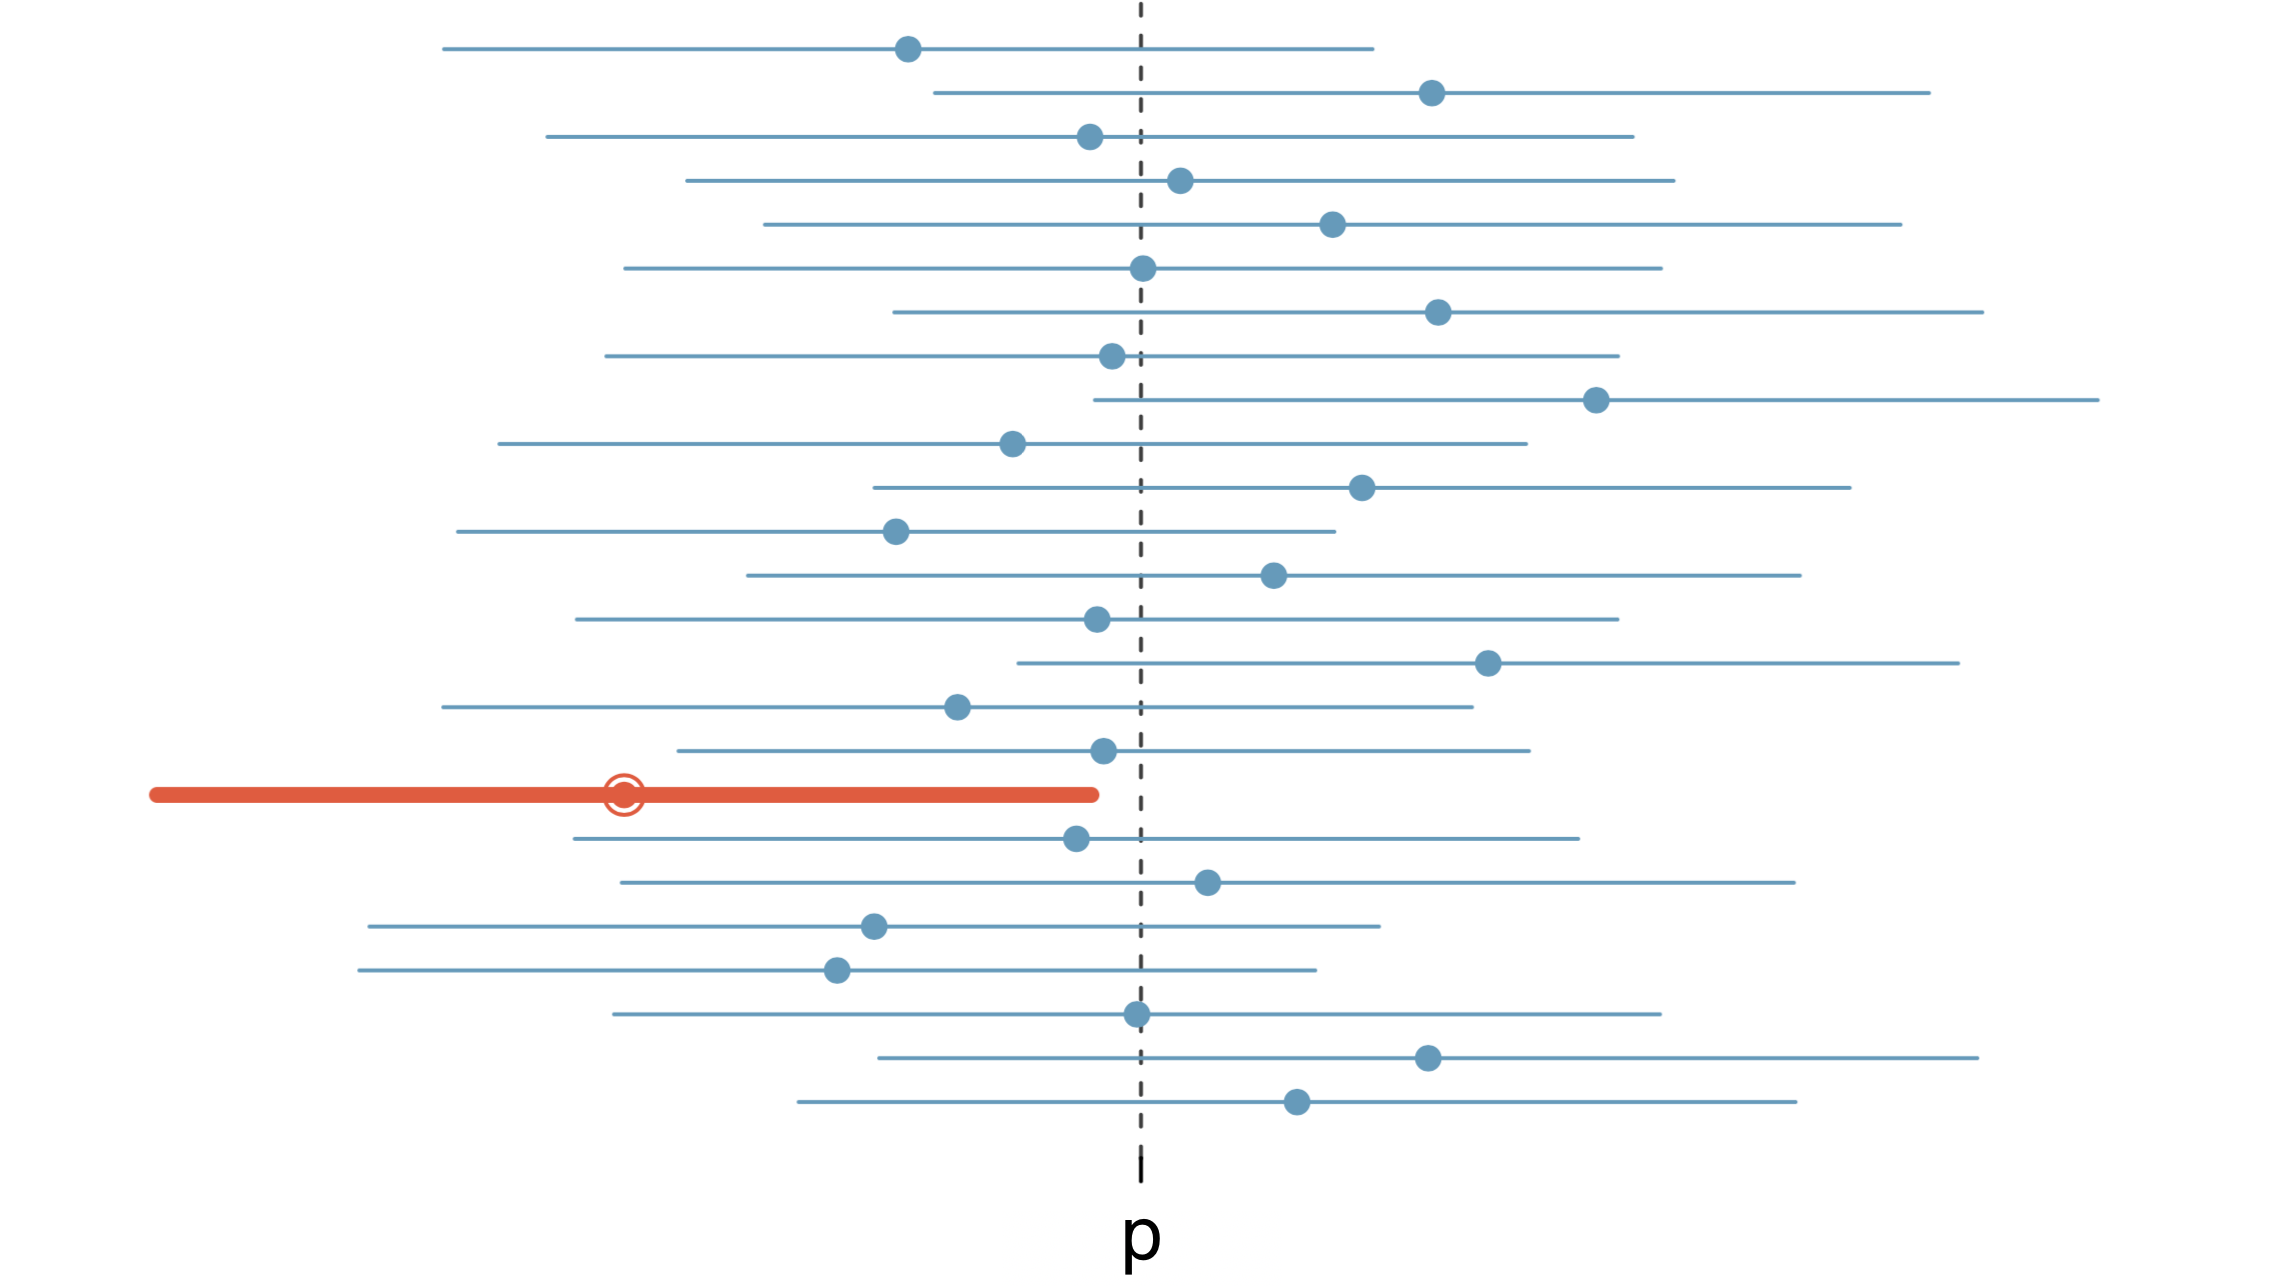
\includegraphics[scale=0.2]{figure/CI.png}
\end{figure}
\end{frame}

%---------------------------------------------
% \begin{frame}
% \begin{itemize}
% \item The interpretation on the previous slide is a bit of a brain twister.
% \item But, technically, it implies that it is incorrect to say that there is a 0.95 probability that the population proportion $p$ is contained in a given interval.
% \item The population proportion $p$ is either contained in a given interval, or it is not.
% \end{itemize}
% \end{frame}

%---------------------------------------------
\begin{frame}{Width of an Interval}
\vspace{-1cm}
If we want to be more certain that we capture the population parameter, i.e. increase our confidence level, should we use a wider interval or a smaller interval?\\
% A wider interval
\vspace{1cm}
Can you think of any drawbacks to using a wider interval?\\

\includegraphics[scale=0.35]{figure/garfield.png}
% If the interval is too wide it may not be very informative
\end{frame}

%---------------------------------------------
\begin{frame}{Changing the Confidence Level}
$$\hat{p} \pm z^* \sqrt{\frac{\hat{p}(1-\hat{p})}{n}}$$
\vspace{10pt}

$z^*$ is called the critical value, which depends on the confidence level (CL).  Some common values are provided in the table below.\\

\vspace{5pt}

\begin{table}[ht]
\begin{tabular}{l|l}
\hline
CL & $z^*$\\
\hline
90\% & 1.645\\
95\% & 1.96\\
99\% &  2.576\\
\hline
\end{tabular}
\end{table}
\end{frame}



%---------------------------------------------
\begin{frame}{Example: Changing the Confidence Level}
\vspace{-3.5cm}
\small
A recent Gallup poll estimated that 56\% of Americans approved of the way Joe Biden is handling his job as president.  The results were based on a random sample of 1,202 American adults.  Calculate a 99\% confidence interval for the population proportion of American adults that approve of Joe Biden.\\
\end{frame}

%---------------------------------------------
\begin{frame}{Changing the Confidence Level}
\vspace{-3cm}
The value for the critical value $z^*$ can be found manually using the R function \texttt{qnorm()}.\\
\vspace{15pt}

\textbf{Example:} Use R to find the critical value $z^*$ that corresponds with a 98\% confidence level.\\

\end{frame}



%---------------------------------------------
\begin{frame}{Terminology}
$$\hat{p} \pm z^* \sqrt{\frac{\hat{p}(1-\hat{p})}{n}}$$
\begin{itemize}
\item $z^*$ is called the \textbf{critical value}, which depends on the confidence level
\vspace{10pt}
\item $\sqrt{\frac{\hat{p}(1-\hat{p})}{n}}$ is called the \textbf{standard error} (SE)
\vspace{10pt}
\item $z^* \sqrt{\frac{\hat{p}(1-\hat{p})}{n}}$ is called the \textbf{margin of error} 
\end{itemize}
\end{frame}


%---------------------------------------------
\begin{frame}{Sample Size Determination}
Determine the sample size needed so that the confidence interval will have a margin of error of $\pm E$
\vspace{4cm}

\small
\begin{itemize}
\item If no data has been collected then use $\hat{p} = 0.5$, which gives the largest possible sample size.
\item When an estimate of the proportion is available, use it in place of 0.5.
\end{itemize}
\end{frame}

\begin{frame}{Example: Sample Size Determination}
\vspace{-3.5cm}
A university newspaper is conducting a survey to determine what percentage of students support an increase in fees to pay for a new football stadium.  How big of a sample is needed so that the margin of error is $\pm 0.04$ using a 95\% confidence level?\\
\end{frame}


\end{document}
